% !TEX encoding = UTF-8 Unicode

%
% Exemple de rapport
% par Pierre Tremblay, Universite Laval
% modifié par Christian Gagne, Universite Laval
% modifié par Francis Valois, Université Laval
% 31/01/2011 - version 1.4
%

%
% Modele d'organisation d'un projet LaTeX 
% rapport/      dossier racine et fichier principal
% rapport/fig   fichiers des figures
% rapport/tex   autres fichiers .tex
%

% ** Preambule **
%
% Ajouter les options au besoin :
%    - "ULlof" pour inclure la liste des figures, requis si "\begin{figure}" utilise
%    - "ULlot" pour inclure la liste des tableaux, requis si "\begin{table}" utilise
%
\documentclass[12pt,ULlof,ULlot]{ULrapport}

% Chargement des packages supplementaires (si absent de la classe)
\usepackage[utf8]{inputenc}
\usepackage{array}
\usepackage[T1]{fontenc}
\usepackage[autolanguage]{numprint}
\usepackage{icomma}
\usepackage{subfigure}
\usepackage{graphicx}
\usepackage[absolute]{textpos}
\usepackage[final]{pdfpages}
\usepackage{lscape}
\usepackage{fancyhdr}
\usepackage[onehalfspacing]{setspace}
\usepackage[framed,numbered,autolinebreaks,useliterate]{mcode}
\def\dbar{{\mathchar'26\mkern-12mu d}}
\usepackage{titlesec}
\setlength\aftertitleunit{\baselineskip}

\titleformat{\chapter}[display]
  {\normalfont\Huge \scshape}{\titlerule}{-38pt}{\Huge}[\vspace{-2pt}\titlerule]
\titleformat{name=\chapter,numberless}[display]
  {\normalfont\Huge \scshape}{\titlerule}{-38pt}{\Huge}[\vspace{-2pt}\titlerule]
\titlespacing*{\chapter}{0pt}{0pt}{*2} 
%\usepackage[options]{nom_du_package}

% Definition d'une commande pour presenter des cellules multilignes dans un tableau
\newcommand{\cellulemultiligne}[1]{\begin{tabular}{@{}c@{}}#1\end{tabular}}


% Definition de colonnes en mode paragraphe avec alignement ajustable
% Cette definition requiert le chargement du package "array"
%    - alignement horizontal, parametre #1 : - \raggedright (aligne a gauche)
%                                            - \centering (c\item $K_D = 14.70$entre)
%                                            - \raggedleft (aligne a droite)
%    - alignement vertical, parametre #2 : - p (aligne en haut)
%                                          - m (centre)
%                                          - b (aligne en bas)
%    - largeur, parametre #3 : longueur
\newcolumntype{Z}[3]{>{#1\hspace{0pt}\arraybackslash}#2{#3}}

% Definitions des parametres de la page titre
\TitreProjet{Simulation d’une alimentation des électroaimants d’un accélérateur de particules }                         % Titre du projet
\TitreRapport{Design IV - GEL-3005}       % Titre du rapport
\Destinataire{M. Robert Bergevin et M. Jérôme Cros}         % Nom(s) du destinataire
\TableauMembres{%           
   910\,010\,418  & Gabriel Boivin-Desjardins \\\hline                          % Tableau des membres de l'equipe
   910\,055\,897  & Daniel Thibodeau \\\hline
   910\,097\,879  & Francis Valois \\\hline        % matricule & nom & \\\hline
           % matricule & nom & \\\hline     % matricule & nom & \\\hline
}
\DateRemise{28 avril 2014}                           % Date de remis


% Corps du document

\begin{document}
\tableofcontents
\listoffigures
%   Chapitres

\chapter{Introduction}
Les recherches sur la physique fondamentale requièrent des installations hors normes, défiant les limites de ce que l'on considère comme possible. Les installations du CERN, laboratoire européen situé en Suisse qui pratique des expériences à la fine pointe de la technologie est un laboratoire dont le financement est de nature publique et dont la connaissance est diffusée. Une représentation de l'ensemble de l'installation est présentée à la figure \ref{CERN} Ce laboratoire utilise des techniques existantes, mais repousse les limites de précision et de fiabilité. Le sujet d'étude de ce projet de fin d'études porte sur une alimentation électronique visant à remplacer une alimentation existante. Le remplacement doit permettre une augmentation substantielle de l'énergie des faisceaux de protons. Le rôle de l'équipe Électrosim consiste à reproduire l'alimentation en développement au CERN sur  trois simulateurs: SimPowerSystems (SPS), PSIM ainsi que sur un simulateur temps réel, fourni par la compagnie Opal-RT. Le client direct du projet est le laboratoire LEEPCI, de l'Université Laval, qui désire d'une part, étudier la méthode d'implantation de l'alimentation électronique du CERN en la reproduisant sur trois plateformes de simulation et d'autres part, valider l'implantation des modèles de simulations en comparant les résultats sur les différentes plateformes. Le projet vise à obtenir une compréhension théorique des choix techniques effectués par les ingénieurs du CERN en étudiant les résultats de simulation. Le rapport de détaille en plusieurs sections: soit une explication détaillée du contexte et de la problématique entourant l'alimentation électronique, une énumération des besoins et des objectifs rattachés au projet, une présentation du cahier des charges sous le format d'un diagramme des propriétés fonctionnelles,   l'explication de la méthodologie employée, une analyse simplifiée des sous-systèmes implantés et une analyse détaillée du système intégré

\begin{figure}[htb]
\centering
\makebox[\textwidth][c]{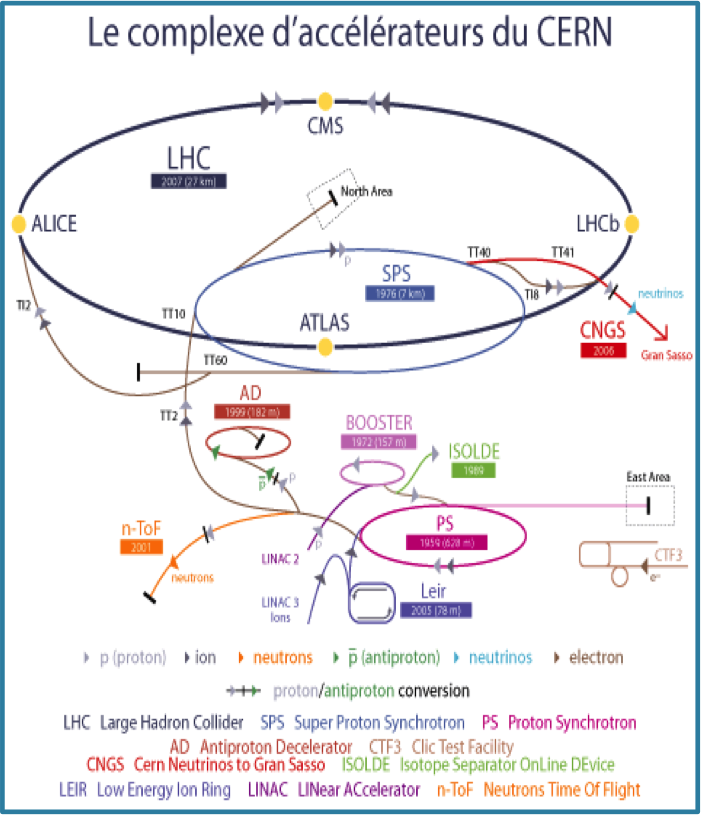
\includegraphics[scale=0.8]{fig/CERN.png}}
\caption{Représentation schématique de l'implantation du complexe d'accélérateurs du CERN}
\label{CERN}
\end{figure}

\chapter{Contexte et problématique}

\chapter{Besoins et objectifs}
Les objectifs du projet portent sur plusieurs volets. Premièrement, il est nécessaire de considérer l'aspect de paramétrisation des simulations et de dimensionnement des composantes employées selon un cahier des charges précis. En ce qui attrait à l'outil de dimensionnement à proprement parler l'outil de paramétrisation et de contrôle, consiste à fournir un outil de contrôle vérifier le dimensionnement des composantes, qui devra être calculé de manière théorique et approximative. Les objectifs à cet endroit sont de:

\begin{itemize}
\item Fournir un outil de dimensionnement pour chaque plateforme qui soit convivial et facile d'utilisation;
\item Livrer un outil de dimensionnement pour chaque plateforme qui utilise les paramètres usuels de nomenclature utilisés dans les simulateurs.
\end{itemize}

\paragraph{}Deuxièmement, pour ce qui est des simulateurs pour chacune des plateforme, il se doivent de:
\begin{itemize}
\item Valider que la conception choisie est fonctionnelle;
\item Permettre la comparaison des résultats de simulation pour différents paramètres de dimensionnement.
\end{itemize}
\paragraph{}Les plateformes sur lesquelles les simulations doivent être livrées sont Simulink(SimPowerSystems), PSIM et Opral-RT. SPS est un outil de simulation générique qui permet de simuler tout type de circuits, toutefois ce côté générique cause des temps de simulation généralement plus longs pour une même précision comparé à des simulateurs spécifiques comme PSIM. L'usage de SPS est problématique au niveau des variations rapides. PSIM est spécialement conçu pour les circuits d'électronique de puissance et de contrôles de moteur, tandis que les simulateurs génériques sont conçus pour les circuits électriques de base. Cet outil permet une meilleure rapidité et une meilleure précision. Par ailleurs, il est plus robuste aux variations rapides. Le simulateur OPA-4500 de Opal-RT est un simulateur temps réel qui permet une comparaison directe des résultats avec SPS. Les pas de simulations sont généralement faible, compte tenu de l'optimisation effectuée et de la puissance des composantes. Cet outil permet de réaliser des simulations en temps réel à partir de SPS. Par ailleurs, l'utilisation d'un simulateur temps réel présente la possibilité de tests d'intégration en temps réel

\paragraph{}Troisièmement, en ce qui attrait à la documentation technique, elle présente d'une part les résultats de calculs de dimensionnement théoriques, d'autres part un guide d'utilisation des simulations et de l'outil de contrôle. L'objectif de cette documentation est donc de:
\begin{itemize}
\item Présenter des exemples d'utilisation des simulations et de l'outil de contrôle et de dimensionnement.
\end{itemize}
\paragraph{}La validation croisée des simulations est nécessaire afin de juger de la validité des résultats, à cet effet, il est donc nécessaire d':
\begin{itemize}
\item Implanter une validation croisées des 3 simulateurs.
\end{itemize}
\newpage
\newlength{\hcolw}
\setlength{\hcolw}{\textwidth}
\eject \pdfpagewidth=11in \pdfpageheight=8.5in
\textwidth=8.5in
\titlespacing{\chapter}{0pt}{-40pt}{10pt}
\chapter{Diagramme des propriétés fonctionnelles}
\begin{table}[h]
\centering
\scalebox{0.5}{
\begin{tabular}{|>{\arraybackslash}m{3in}|>{\centering\arraybackslash}m{1in}|>{\centering\arraybackslash}m{1in}|>{\centering\arraybackslash}m{1in}|>{\centering\arraybackslash}m{1in}|>{\centering\arraybackslash}m{1in}|>{\centering\arraybackslash}m{1in}|>{\centering\arraybackslash}m{1in}|>{\centering\arraybackslash}m{1in}|>{\centering\arraybackslash}m{1in}|>{\centering\arraybackslash}m{1in}|>{\centering\arraybackslash}m{1in}|>{\centering\arraybackslash}m{1in}|>{\centering\arraybackslash}m{1in}|}
\hline
\multirow{12}*{Exigences du client}                                                                                                                                 & \multicolumn{13}{|c|}{Fonctionnalités}                                                                                                                                                                                                                                                                                                                                                                                                                                                                         \\ \cline{2-14} 
                                                                                                                                                                     & \multicolumn{13}{|c|}{Simulateurs}                                                                                                                                                                                                                                                                                                                                                                                                                                                                             \\ \cline{2-14} 
                                                                                                                                                                     & \multicolumn{1}{|c|}{\multirow{6}{1in}{Accepter des paramètres de modélisation}} & Abaisser la tension du réseau alternatif & \multicolumn{4}{|c|}{Redresser le signal d'entrée à la sortie du transformateur}                       & Commander un onduleur triphasé 3 niveaux de type NPC 		   & Charger un banc de condensateur & Commander un convertisseur CC-CC à 4 quadrants multicellules & \multicolumn{3}{|>{\centering\arraybackslash}p{3.2in}|}{ Alimenter les électroaimants de l'accélérateur de particules}  & Afficher des résultats de simulation personnalisés \\ \cline{3-14} 
                                                                                                                                                                     &                                                          						   & Ratio de transformation (\%)             & Ondulation de tension (\%) & Déphasage du courant (°) & Puissance moyenne (MW) & Puissance crête (MW)  & Fréquence tension ligne-ligne (Hz)                   		   & Temps de charge (s)             & Fréquence tension à la charge (Hz)                           & Ondulation de courant (A)    & Puissance moyenne (MW)    & Puissance crête (MW)    & Convivialité (1 à 5)                               \\ \hline
Modéliser une cellule de base d'un onduleur triphasé à 3 niveaux de type NPC                                                                                         & 5                                                        						   &                                          & 5                          & 5                        & 5                      & 5                     & 3                                                    		   &                                 & 5                                                            & 3                            & 3                         & 3                      &                                                    \\ \hline
Modéliser la commande dans le cas de l'onduleur de type AFE.                                                                                                         & 5                                                        						   &                                          & 5                          & 5                        & 5                      & 5                     & 5                                                    		   &                                 & 5                                                            & 3                            & 3                         & 3                       &                                                    \\ \hline
Implanter le modèle de la configuration de base d'un onduleur triphasé à 3 niveaux NPC dans un simulateur                                                            & 5                                                        						   &                                          & 5                          & 5                        & 5                      & 5                     & 3                                                    		   &                                 & 5                                                            & 3                            & 3                         & 3                       &                                                    \\ \hline
Implanter le modèle de la commande dans le cas de l'onduleur de type AFE dans un simulateur                                                                          & 5                                                                                &                                          & 5                          & 5                        & 5                      & 5                     & 5                                                   		   &                                 & 5                                                            & 3                            & 3                         & 3                       &                              						\\ \hline
Fournir un outil de dimensionnement pour l'onduleur de type AFE                                                                                                      & 2                                                        						   &                                          & 2                          & 2                        & 2                      & 2                     & 2                                                    		   & 2                               & 2                                                            & 2                            & 2                         &2                       & 3                                                  \\ \hline
Modéliser un convertisseur CC-CC à 4 quadrants à l'aide de plusieurs cellules de type onduleur NPC                                                                   & 5                                                        						   &                                          &                            &                          &                        &                       &                                                     		   &                                 & 5                                                            & 5                            & 5                         &5                      &						                            \\ \hline
Modéliser la commande d'un convertisseur CC-CC à 4 quadrants                                                                                                         & 5                                                        						   &                                          &                            &                          &                        &                       &                                                     		   &                                 & 5                                                            & 5                            & 5                         &5                      & 						                             \\ \hline
Implanter le modèle d'un convertisseur CC-CC à 4 quadrants à l'aide de plusieurs cellules de type onduleur NPC avec des inductances de découplage dans un simulateur & 5                                                        						   &                                          &                            &                          &                        &                       &                                                      		   &                                 & 5                                                            & 5                            & 5                         &5                       &                                                    \\ \hline
Implanter le modèle de la commande d'un convertisseur CC-CC à 4 quadrants alimentant la charge spécifiée dans un simulateur                                          & 5                                                       						   &                                          &                            &                          &                        &                       &                                                     		   &                                 & 5                                                            & 5                            & 5                         & 5                       &                                                    \\ \hline
Fournir un outil de dimensionnement pour le convertisseur CC-CC  à 4 quadrants                                                                                       & 2                                                        						   &                                          &                            &                          &                        &                       &                                                     		   & 2                               & 2                                                            & 2                            & 2                         & 2                       & 3                                                  \\ \hline
Implanter le modèle complet de l'alimentation du Booster dans un simulateur                                                                                          & 5                                                        						   & 5                                        &                            &                          &                        &                       &                                                     		   & 5                               & 5                                                            & 5                            & 5                         & 5                       & 5                                                  \\ \hline
Effectuer la validation croisée des configurations implantées à l'aide de 3 simulateurs (PSIM, SimPowerSystems, Opal-RT)                                             & 5                                                       						   & 3                                        & 5                          & 5                        & 5                      & 5                     & 5                                                   		   & 3                               & 5                                                            & 5                            & 5                         & 5                       & 5                                                  \\ \hline
Livrer une documentation pédagogique pour les divers outils de dimensionnement et de simulation                                                                      & 4                                                       						   &                                          &                            &                          &                        &                       &                                                      		   &                                 &                                                              &                              &                           &                                              & 4                                                  \\ \hline
\end{tabular}}
\caption{Première partie du diagramme des propriétés fonctionnelles (DPF)}
\end{table}
\clearpage

% Please add the following required packages to your document preamble:
% \usepackage{multirow}

\begin{table}[ht]
\centering
\scalebox{0.6}{
\begin{tabular}{|>{\arraybackslash}m{3in}|>{\centering\arraybackslash}m{1in}|>{\centering\arraybackslash}m{1in}|>{\centering\arraybackslash}m{1in}|>{\centering\arraybackslash}m{1in}|>{\centering\arraybackslash}m{1in}|>{\centering\arraybackslash}m{1in}|>{\centering\arraybackslash}m{1in}|>{\centering\arraybackslash}m{1in}|>{\centering\arraybackslash}m{1in}|}
\hline
\multirow{11}{3in}{Exigences du client}                                                                                                                                 & \multicolumn{9}{|c|}{Fonctionnalités}                                                                                                                                                                                                                                                                                                                                                                                                                                                   \\ \cline{2-10} 
                                                                                                                                                                     & \multicolumn{2}{|c}{Outil de dimensionnement}                                                                         & \multicolumn{7}{|c|}{Documentation}                                                                                                                                                                                                                                                                                                                             \\ \cline{2-10} 
                                                                                                                                                                     & Accepter des paramètres de dimensionnement usuels & Fournir les paramètres de modélisation utilisés par le simulateur & \multicolumn{2}{|>{\centering\arraybackslash}m{2.2in}|}{Présenter le fonctionnement de l'outil de dimensionnement de chacun des simulateurs} & Présenter les modèles mathématiques utilisés dans chacun des simulateurs & \multicolumn{2}{|>{\centering\arraybackslash}m{2.2in}}{Présenter l'utilisation de chacun des simulateurs} & \multicolumn{2}{|>{\centering\arraybackslash}m{2.2in}|}{Présenter les procédures de validation croisées de chacun des simulateurs} \\ \cline{2-10} 
                                                                                                                                                                     & Choix disponibles (1 à 5)                         & Convivialité (1 à 5)                                              & Précision de l'information (1 à 5)                         & Convivialité (1 à 5)                         &                                                                          & Précision de l'information (1 à 5)        & Convivialité (1 à 5)       & Précision de l'information (1 à 5)                    & Convivialité (1 à 5)                    \\ \hline
Modéliser une cellule de base d'un onduleur triphasé à 3 niveaux de type NPC                                                                                         & 5                                                 & 3                                                                 &                                                            &                                              & 5                                                                        &                                           &                            &                                                       &                                         \\ \hline
Modéliser la commande dans le cas de l'onduleur de type AFE.                                                                                                         & 5                                                 & 3                                                                 &                                                            &                                              & 5                                                                        &                                           &                            &                                                       &                                         \\ \hline
Implanter le modèle de la configuration de base d'un onduleur triphasé à 3 niveaux NPC dans un simulateur                                                            & 3                                                 & 5                                                                 & 3                                                          & 3                                            &                                                                          & 4                                         & 4                          & 4                                                     & 4                                       \\ \hline
Implanter le modèle de la commande dans le cas de l'onduleur de type AFE dans un simulateur                                                                          & 3                                                 & 5                                                                 & 3                                                          & 3                                            &                                                                          & 4                                         & 4                          & 4                                                     & 4                                       \\ \hline
Fournir un outil de dimensionnement pour l'onduleur de type AFE                                                                                                      & 5                                                 & 5                                                                 & 5                                                          & 5                                            &                                                                          &                                           &                            &                                                       &                                         \\ \hline
Modéliser un convertisseur CC-CC à 4 quadrants à l'aide de plusieurs cellules de type onduleur NPC                                                                   & 5                                                 & 3                                                                 &                                                            &                                              & 5                                                                        &                                           &                            &                                                       &                                         \\ \hline
Modéliser la commande d'un convertisseur CC-CC à 4 quadrants                                                                                                         & 5                                                 & 3                                                                 &                                                            &                                              & 5                                                                        &                                           &                            &                                                       &                                         \\ \hline
Implanter le modèle d'un convertisseur CC-CC à 4 quadrants à l'aide de plusieurs cellules de type onduleur NPC avec des inductances de découplage dans un simulateur & 3                                                 & 5                                                                 & 3                                                          & 3                                            &                                                                          & 4                                         & 4                          & 4                                                     & 4                                       \\ \hline
Implanter le modèle de la commande d'un convertisseur CC-CC à 4 quadrants alimentant la charge spécifiée dans un simulateur                                          & 3                                                 & 5                                                                 & 3                                                          & 3                                            &                                                                          & 4                                         & 4                          & 4                                                     & 4                                       \\ \hline
Fournir un outil de dimensionnement pour le convertisseur CC-CC  à 4 quadrants                                                                                       & 5                                                 & 5                                                                 & 5                                                          & 5                                            &                                                                          &                                           &                            &                                                       &                                         \\ \hline
Implanter le modèle complet de l'alimentation du Booster dans un simulateur                                                                                          & 3                                                 & 5                                                                 & 3                                                          & 3                                            & 5                                                                        & 5                                         & 5                          & 5                                                     & 5                                       \\ \hline
Effectuer la validation croisée des configurations implantées à l'aide de 3 simulateurs (PSIM, SimPowerSystems, Opal-RT)                                             &                                                   &                                                                   &                                                            &                                              &                                                                          &                                           &                            & 5                                                     & 5                                       \\ \hline
Livrer une documentation pédagogique pour les divers outils de dimensionnement et de simulation                                                                      & 4                                                 & 4                                                                 & 5                                                          & 5                                            & 5                                                                        & 5                                         & 5                          & 5                                                     & 5                                       \\ \hline
\end{tabular}}
\caption{Seconde partie du diagramme des propriétés fonctionnelles (DPF)}
\end{table}
\eject \pdfpagewidth=8.5in \pdfpageheight=11in
\textwidth=\hcolw
\chapter{Méthodologie}
La méthodologie employée pour ce projet est une approche qui vise à fragmenter le système en sous-systèmes simples, plus faciles à analyser et qui permet par la suite de construire une expertise servant à intégrer les notions propres au concept complet. Concrètement, il faut:
\begin{itemize}
\item Modéliser le redresseur NPC 3 niveaux à 3 bras par un redresseur actif triphasé (AFE);
\item Modéliser le hacheur 4 quadrants simplifié à 4 interrupteurs (de manière préliminaire);
\item Modéliser le hacheur 4 quadrants avec 2 cellules NPC 3 niveaux à commande entrelacée.
\end{itemize}
\paragraph{} Les simulations résultantes sont premièrement modélisées par des systèmes indépendants en boucle ouverte et par la suite par des systèmes en boucle fermée avec des régulateurs. Les sous-systèmes du projet sont les suivants:
\begin{itemize}
\item Modélisation simplifiée de la régulation de tension de l'AFE par un redresseur 2 niveaux débitant sur une charge idéale avec régulation d'angle et de courant par hystérésis, permettant le fonctionnement 4 quadrants du redresseur actif;
\item Modélisation simplifiée de la régulation de tension  de l'AFE par un redresseur 2 niveaux débitant sur une charge RC initialement chargée avec facteur de puissance unitaire imposé et régulation de courant par hystérésis;
\item Modélisation de l'AFE 3 niveaux NPC  débitant sur une charge RC initialement chargée avec facteur de puissance unitaire imposé et régulation de courant par MLI;
\item Modélisation du convertisseur CC-CC 4 quadrants par un hacheur 4 quadrants simple formé de 4 interrupteurs, alimenté à partir d'une charge idéale et commandé par MLI à 1kHz;
\item Modélisation du convertisseur CC-CC 4 quadrants par un hacheur formé de 2 cellules onduleur NPC 3 niveaux triphasées avec inductances de couplage, alimenté avec une source idéale et commandée par MLI décalée à 333Hz.
\end{itemize}

Le reste de la méthodologie consiste à assembler les différents sous-systèmes sous 3 plateformes distinctes. Il est donc nécessaire de:
\begin{itemize}
\item Valider les fonctionnalités des systèmes reliés;
\item Valider la concordance des résultats de simulations sous 3 plateformes.
\end{itemize}

Ce qui résulte de cette méthodologie est une intégration graduelle de la complexité des modèles, d'une part avec un développement un boucle ouverte, puis un développement en boucle fermée. Les systèmes sont par la suite corrélés sur les différentes plateformes, puis intégrés en sous-systèmes de complexité supérieure. Le tout est par la suite validé sur les différentes plateformes de simulation.
%!TEX root = ../rapport.tex
%!TEX encoding = UTF-8 Unicode
\chapter{Outil de contrôle et de dimensionnement}
Cette section présente l'interface de contrôle et de dimensionnement des simulateurs PSim et SPS.

En premier lieu, on doit indiquer à l'outil de contrôle les différentes simulations ainsi que les chemins d'accès respectifs pour y accéder. La figure \ref{outil1} présente les informations nécessaires pour le bon fonctionnement de l'outil.

 \begin{figure}[htb]
 \centering
 \makebox[\textwidth][c]{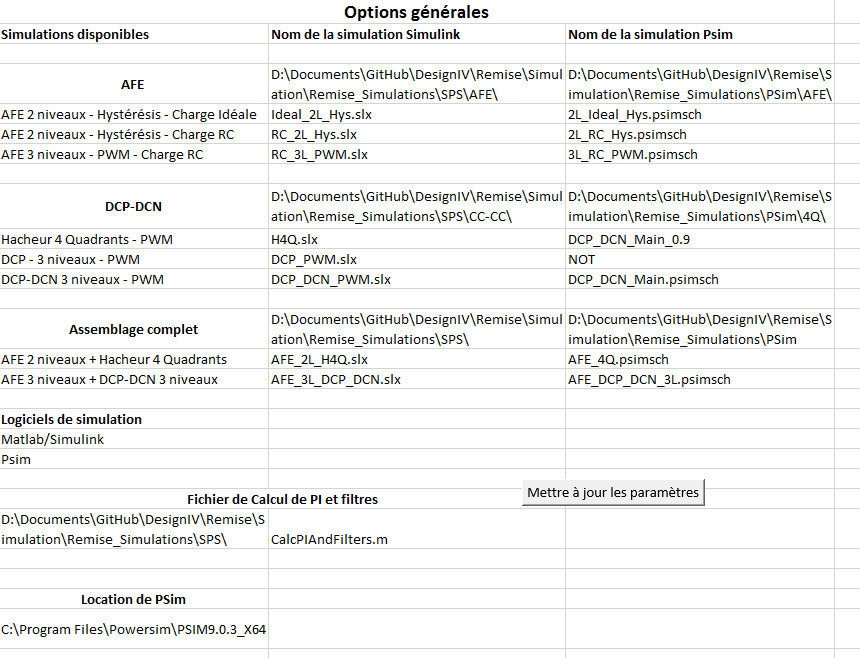
\includegraphics[width=0.95\textwidth]{fig/outil1.png}}
 \caption{Préprogrommation de l'outil de contrôle et de dimensionnement}
 \label{outil1}
 \end{figure}

Une fois les informations des simulations mises en place, il suffit de choisir la simulation à lancer, de choisir le simulateur cible et d'entrer les différents paramètres de simulation. La figure \ref{outil2} présente l'interface de lancement et de programmation des paramètres.

 \begin{figure}[htb]
 \centering
 \makebox[\textwidth][c]{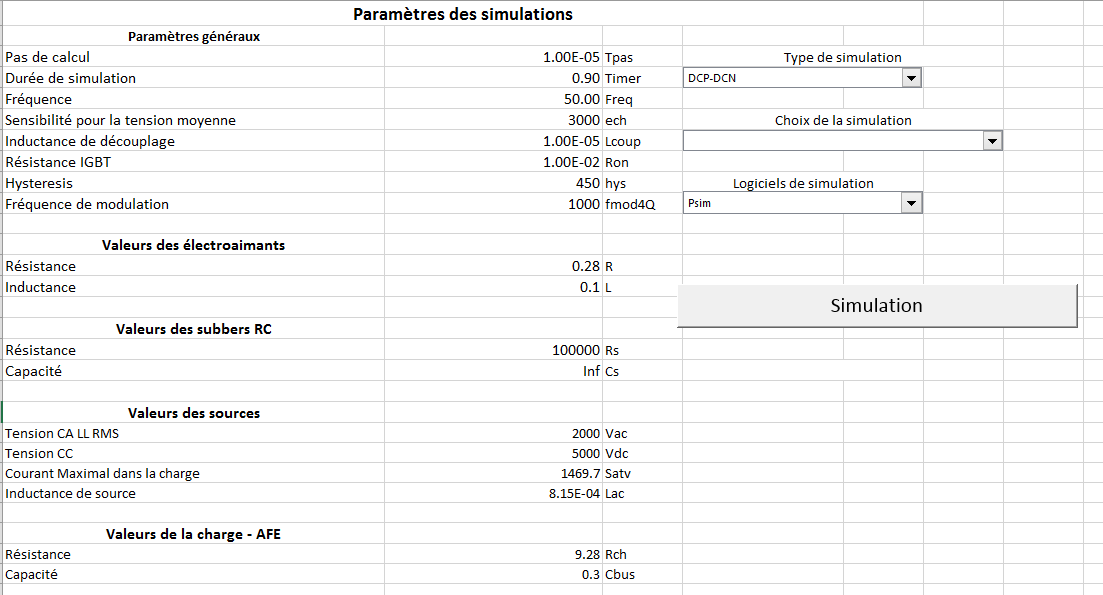
\includegraphics[width=0.95\textwidth]{fig/outil2.png}}
 \caption{Interface de lancement et de programmation des paramètres}
 \label{outil2}
 \end{figure}

 Cet outil permet de gagner un temps précieux lors de l'enchaînement rapide des simulations, car tous les paramètres capitaux sont regroupés au même endroit. De plus, comme l'outil permet de contrôler les deux plateformes de simulation, les valeurs vont être les mêmes d'une plateforme vers l'autre. On s'assure ainsi d'une homogénéité des résultats et on évite des erreurs humaines liées à la manipulation séquentielle des blocs dans les plateformes. 

\chapter{Validation croisée des simulations}
Dans cette section, par souci de simplicité, juste les sous-systèmes avec la configuration finale est exploré. 

\section{Convertisseur CC-CC 4 quadrants formé de 2 convertisseurs 3 niveaux NPC}
Ce sous-système représente le DCP/DCN, le convertisseur CC-CC indiqué sur la figure présenté au début de ce document représentant le schéma complet du système à implémenter. Le fonctionnalité de ce système est de reproduire une forme de courant précise à la charge, il est testé sur source idéal et est capable de  reproduire le courant désirée sur une charge RL comme on le remarque sur la figure~\ref{DC_ch_cou_1}, il n'y a pas de grosse différence entre PSIM et SPS mise à part un décalage en fréquence. La dynamique du système suit très bien la courbe de référence avec une oscillation d'environs 15A. Il y a présence de commutation non désirée mais ça n'affecte pas le fonctionnement du système. 



\begin{figure}[htb]
\centering
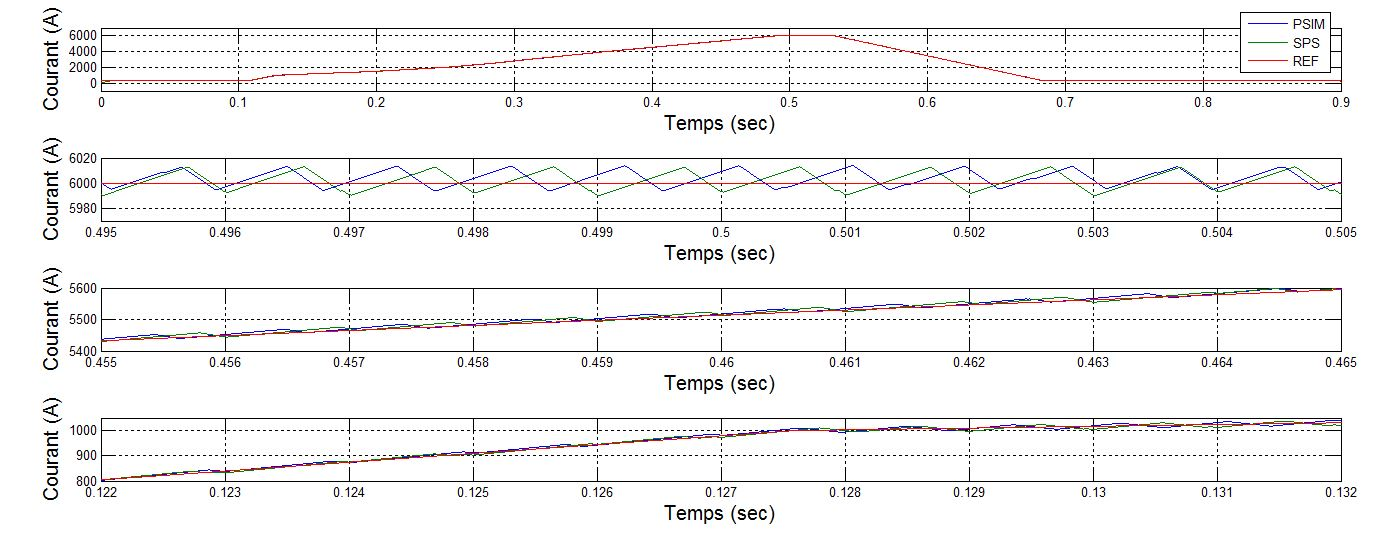
\includegraphics[scale=0.5]{fig/DCPDCN/DCPCourantCharge1u.jpg}
\caption{Courant traversant la charge sur PSIM et SPS pour un pas de calcul de 1$\mu$s pour le DCP/DCN}
\label{DC_ch_cou_1}
\end{figure}

\begin{figure}[htb]
\centering
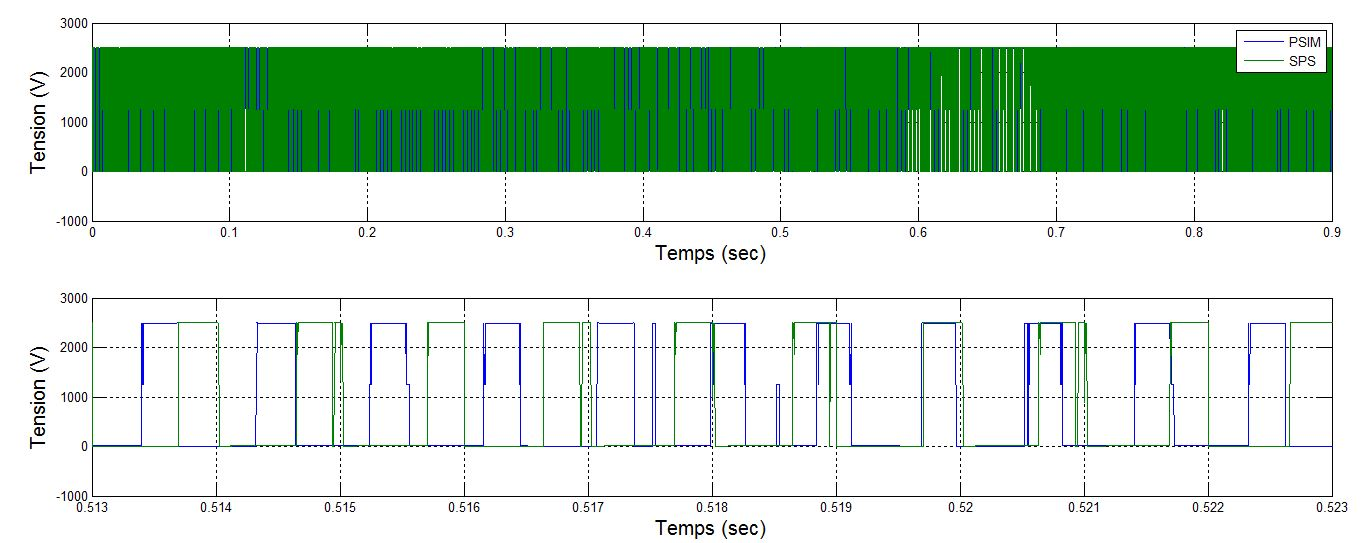
\includegraphics[scale=0.5]{fig/DCPDCN/DCPTensionIGBT1u.jpg}
\caption{Tension aux bornes d'un IGBT sur PSIM et SPS pour un pas de calcul de 1$\mu$s pour le DCP/DCN}
\label{DC_IG_ten_1}
\end{figure}

\clearpage
\section{AFE 3 niveaux NPC avec contrôle par MLI}
Ce sous-système représente l'AFE. Il est testée sur une consigne de tension périodique pour reproduire la dynamique du système. La figure~\ref{AF_RC_cou} montre que le système réagit au changement de consigne de courant de manière identique entre PSIM et SPS. On remarque un décalage entre la courbe de tension de PSIM et SPS tel que vu sur la figure~\ref{AF_RC_ten} d'environs 5V. Dû au nombre élevé de complexité du modèle il est difficile d'indiquer exactement ce qui peut causer cette différence mais on remarque de même un fonctionnement pratiquement identique entre PSIM et SPS. On observe sur la figure~\ref{AF_RC_igbt} que les commutation de SPS et PSIM sont identiques et se déroulent au même moment.


\begin{figure}[htb]
\centering
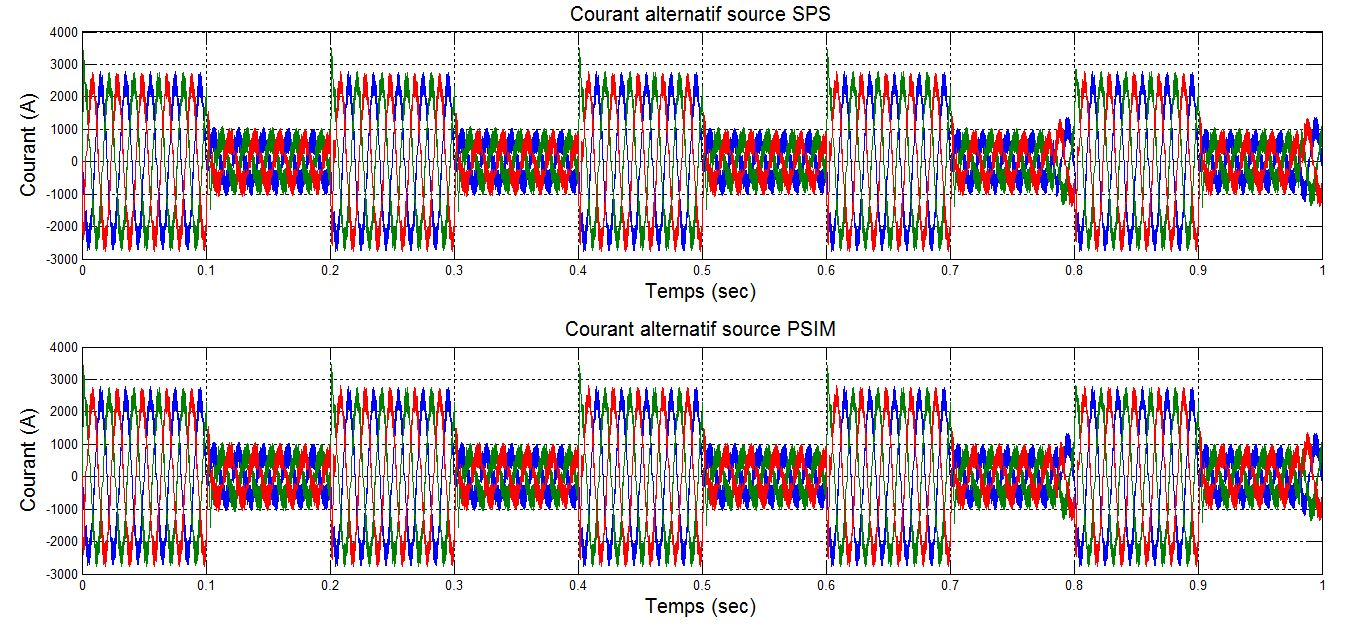
\includegraphics[scale=0.5]{fig/coual_afe.jpg}
\caption{Le courant d'entré à 1$\mu$s pour l'AFE sur charge RC}
\label{AF_RC_cou}
\end{figure}




\begin{figure}[htb]
\centering
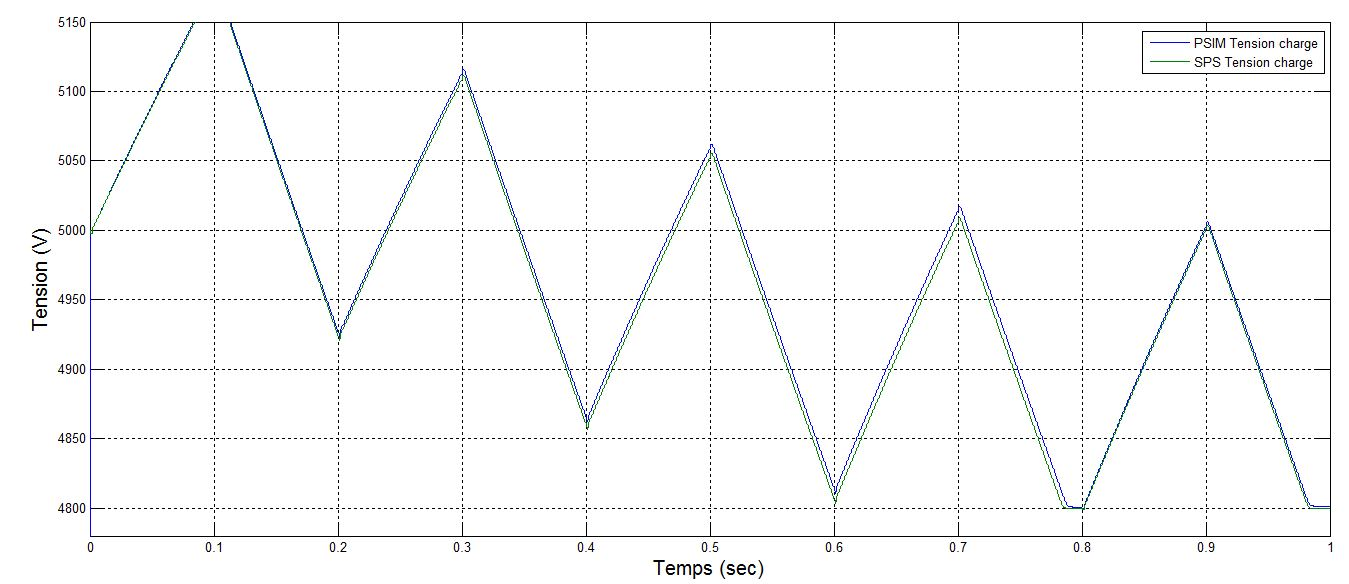
\includegraphics[scale=0.5]{fig/ten_afe.jpg}
\caption{La tension à la charge à 1$\mu$s pour l'AFE sur charge RC}
\label{AF_RC_ten}
\end{figure}



\begin{figure}[htb]
\centering
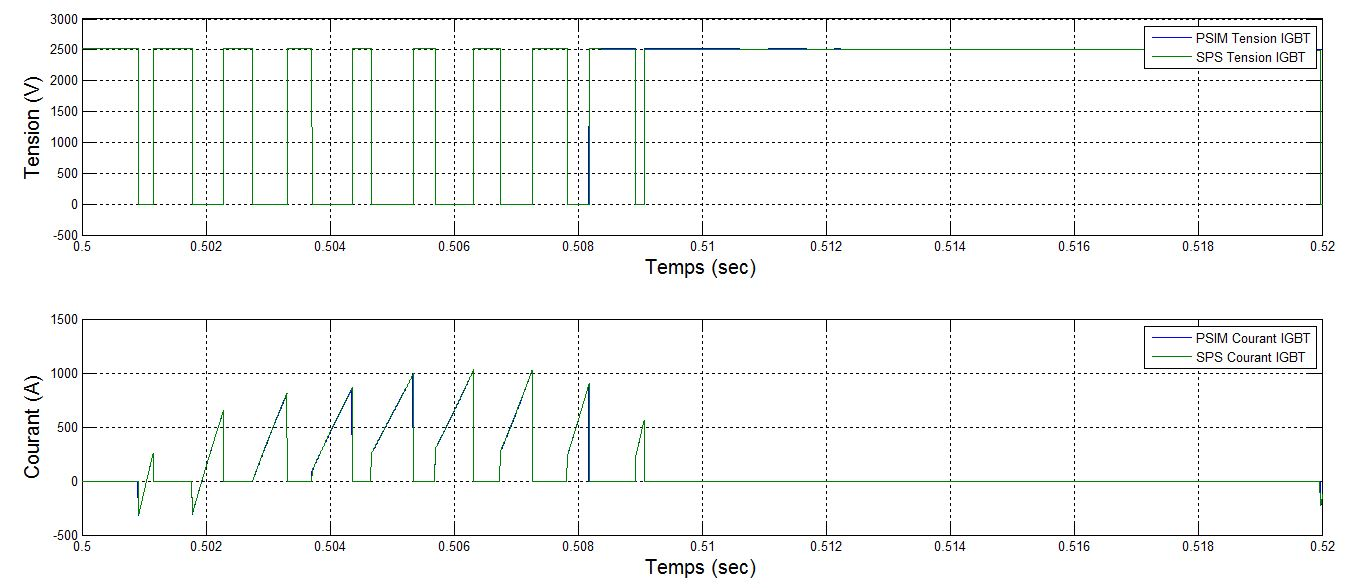
\includegraphics[scale=0.5]{fig/com_afe.jpg}
\caption{La tension et le courant au bornes d'un IGBT à 1$\mu$s pour l'AFE sur charge RC}
\label{AF_RC_igbt}
\end{figure}

\clearpage
\section{AFE 3 niveaux NPC avec contrôle par MLI avec convertisseur CC-CC formé de 2 cellules NPC 3 niveaux}
Ce sous-système représente le système complet, l'intégration de l'AFE et le DCP/DCN. On observe un fonctionnement tout à fait semblable mise à part un décalage d'environs 50V entre PSIM et SPS tel que vu sur la figure~\ref{AF_DC_vch1}. On observe que pour les deux systèmes, soit SPS et PSIM, on arrive à 200V environs de la courbe obtenu par le CERN au niveau de la tension sur le bus CC. Cette différence s'explique par un manque de donnée et d'information par rapport au système complet du CERN. Malgré un manque de donnée, nous réussissons à reproduire la forme de courant désirée~\ref{AF_DC_CHA1}. Une oscillation d'environs 15A est aperçu. Par contre, même si on réussi à limiter la puissance active délivrée du réseau à 3.6MW tel que montré sur la figure~\ref{AF_DC_CHA2}. On observe que PSIM délivre une puissance on peu plus élevé de SPS ce qui fait en sorte que le bus CC finit de se recharger environs 30ms avant sur PSIM que SPS.


\begin{figure}[htb]
\centering
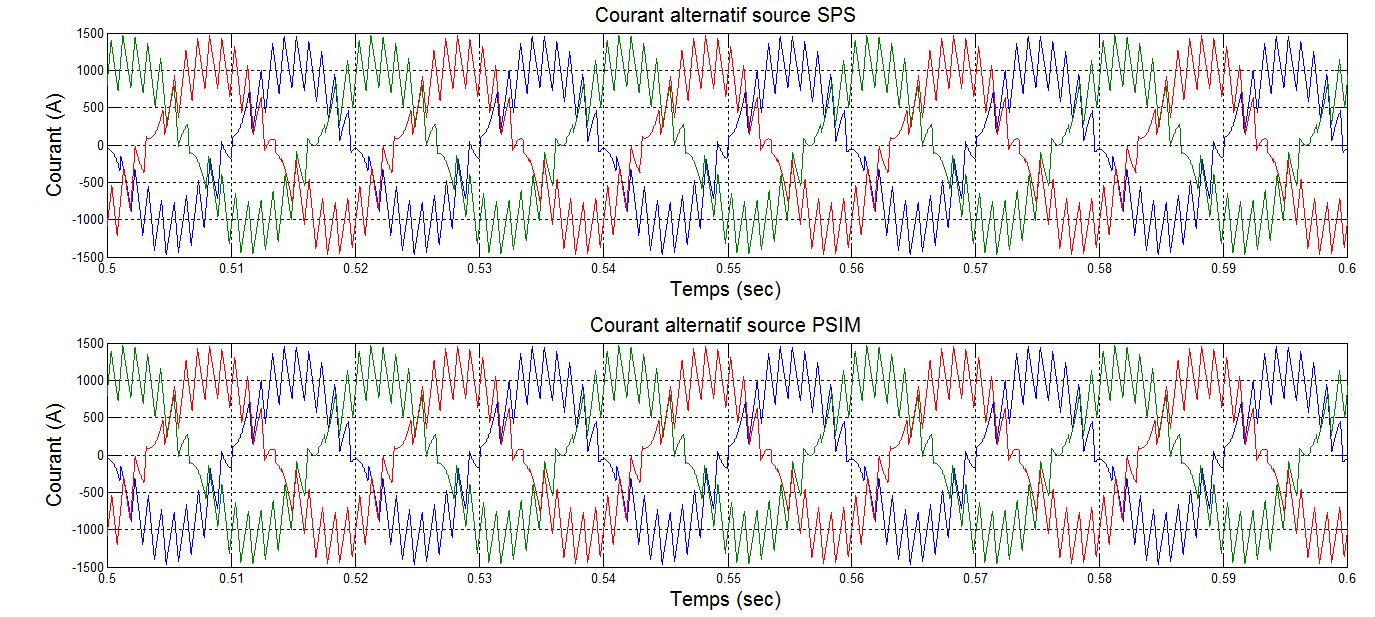
\includegraphics[scale=0.5]{fig/DCP_AFE/1u/cour_al.jpg}
\caption{Le courant d'entrée de l'AFE pour un pas de calcul de 1$\mu$s}
\label{AF_DC_cou1}
\end{figure}


\begin{figure}[htb]
\centering
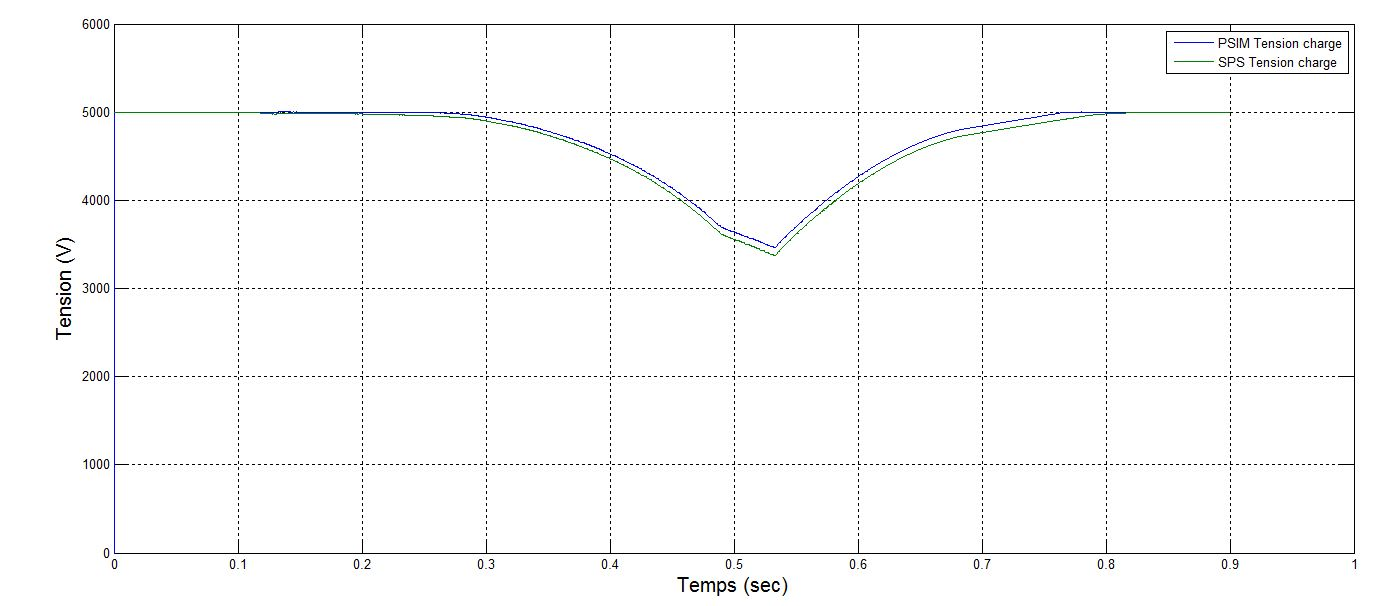
\includegraphics[scale=0.5]{fig/DCP_AFE/1u/ten_bus.jpg}
\caption{La tension du bus CC pour un pas de calcul de 1$\mu$s}
\label{AF_DC_vch1}
\end{figure}

\begin{figure}[htb]
\centering
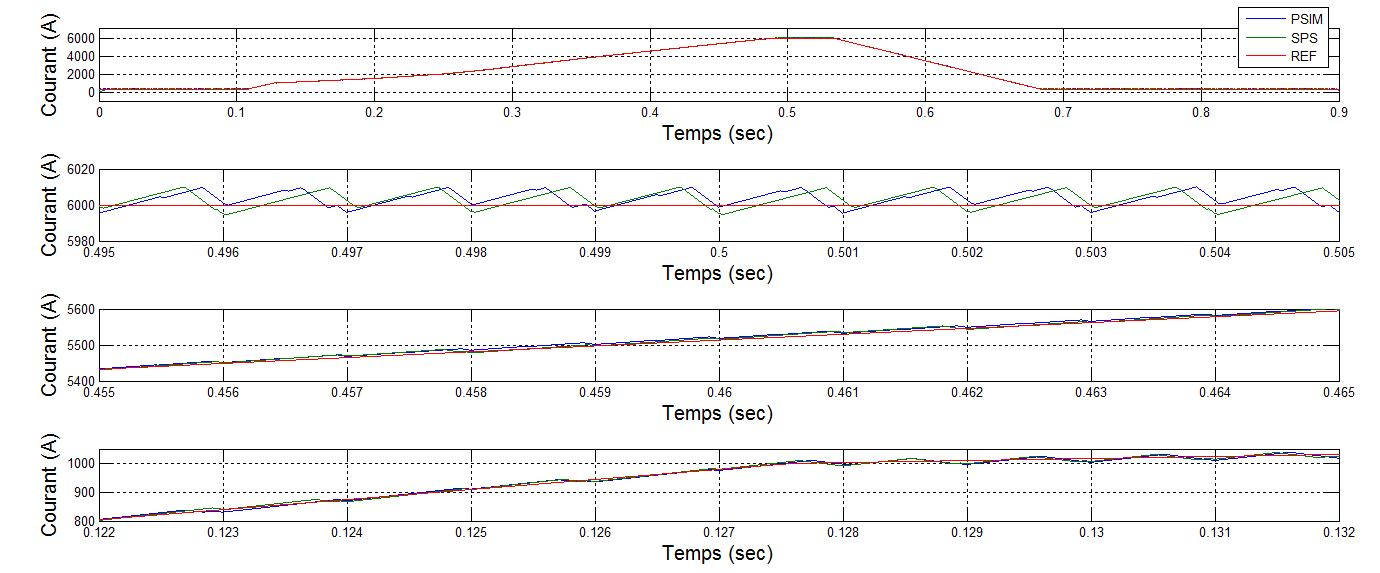
\includegraphics[scale=0.5]{fig/DCP_AFE/1u/cour_ch.jpg}
\caption{Le courant aux bornes des électroaimants pour un pas de calcul de 1$\mu$s}
\label{AF_DC_CHA1}
\end{figure}

\begin{figure}[htb]
\centering
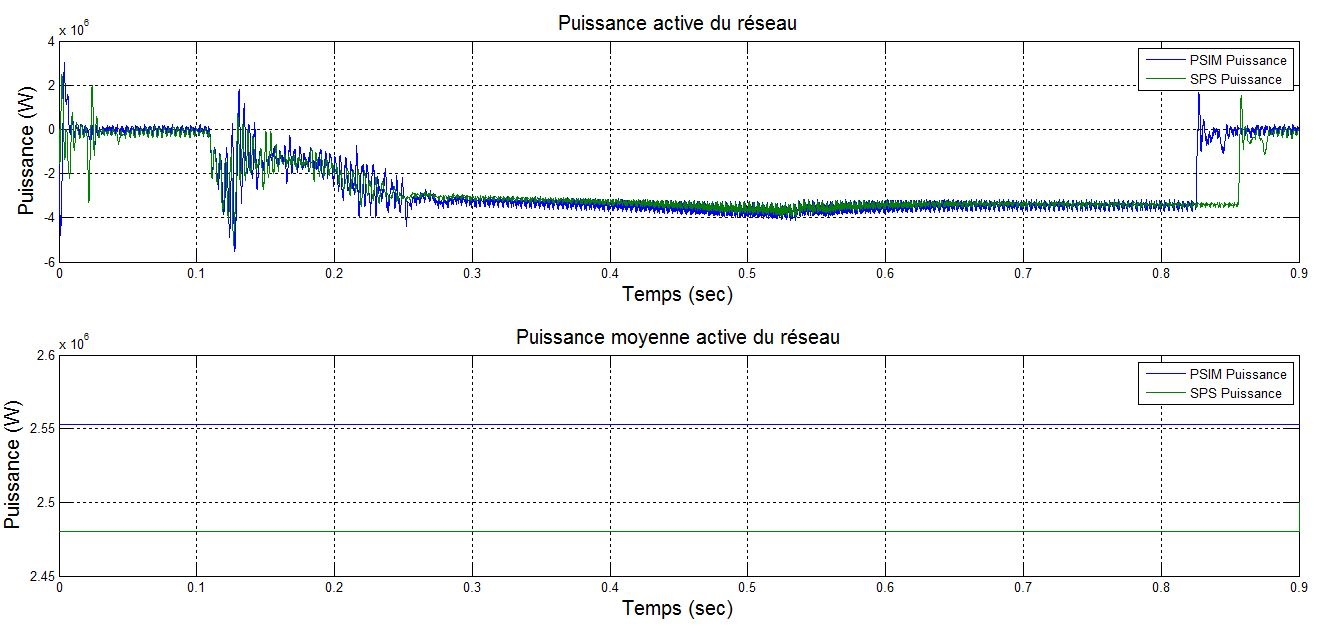
\includegraphics[scale=0.5]{fig/DCP_AFE/1u/PUI.jpg}
\caption{La puissance délivrée par le réseau alternatif pour un pas de calcul de 1$\mu$s}
\label{AF_DC_CHA2}
\end{figure}



%!TEX root = ../rapport.tex
%!TEX encoding = UTF-8 Unicode
\chapter{Simulation temps réel - Opal-RT}
Ce chapitre présente les principaux domaines d'utilisation d'un simulateur temps-réel comme ceux produits par la compagnie Opal-RT ainsi que la validation croisée entre SPS et le simulateur temps réel pour la simulation du hacheur 4 quadrants simple.

\section{Cas typiques d'utilisation d'un simulateur temps-réel}
Le simulateur temps-réel possède trois cas typiques d'utilisation. Premièrement, le simulateur temps-réel permet d'effectuer de la modélisation de type "Hardware-in-the-loop". Dans ce type de simulation, le simulateur temps-réel va modéliser un système tels un réseau électrique de grande envergure, un parc d'éolienne ou l'alimentation d'un appareillage spécifique. À l'aide de cette modélisation et des différents modules d'entrées-sorties du simulateur, il est possible de faire interagir le simulateur directement avec différents modules de contrôle. Ainsi, il n'est pas nécessaire de faire des essais directement sur le réseau ou sur les machines de grosse envergure.

\paragraph{} Deuxièmement, le simulateur temps-réel peut effectuer complètement le contraire. En effet, il suffit d'implanter le module de contrôle à l'intérieur du simulateur et de connecter celui-ci sur le réseau ou sur l'appareillage qui doit être contrôlé pour effectuer les différents essais nécessaires en lien avec le contrôleur.

\paragraph{} Finalement, le troisième cas type est l'assemblage des deux types de simulation. En simulant le contrôle de l'équipement ainsi que l'équipement lui même, il est possible de faire différents essais en peu de temps sachant que le simulateur est capable d'effectuer la simulation en temps réel avec un pas de calcul très petit.

\section{Simulation du hacheur 4 quadrants sur Opal-RT}
Pour effectuer l'implantation du hacheur 4 quadrants sur Opal-RT, plusieurs étapes ont été nécessaires pour obtenir les résultats recherchés. En effet, la suite de logiciels fournie par Opal-RT manque beaucoup de convivialité et la documentation possède beaucoup de zones grises ce qui cause beaucoup d'essais par tâtonnement pour effectuer l'implantation de la simulation. De plus, comme le simulateur doit s'interfacer avec Matlab, celui-ci est dépendant des versions installées. Ainsi, lors de nos différents essais, il a fallu retrouver une version de Matlab 2011b pour que tous les outils d'Opal-RT soient fonctionnels. Une fois les différents logiciels nécessaires installés et fonctionnels, il a été possible d'implanter la simulation du hacheur 4 quadrants en utilisant les renseignements obtenus lors de notre formation sur le simulateur temps réel. Toutefois, effectuer la conversion d'une simulation SPS vers une simulation Opal-RT n'est pas réellement ardu. 

\paragraph{} Une fois venu le temps d'exploiter la simulation, plusieurs pépins ont été rencontrés au niveau de l'affichage des courbes en temps réel ainsi qu'au niveau de la précision des résultats. Il a été nécessaire de jouer avec les paramètres de communication entre Matlab et le simulateur pour obtenir le résultat recherché. Finalement, suite à plusieurs interactions avec l’ assistance technique d'Opal-RT, il a été possible d'obtenir un résultat acceptable. Les figures \ref{DC_ch_H4Q_1} et \ref{DC_ch_H4Q_2} montre le courant obtenu dans l'électroaimant pour un pas de calcul de 25 $\mu$s. On remarque que le simulateur présente la dynamique recherchée. L'ondulation de courant possède une fréquence d'environ 1 kHz comme spécifié et le courant possède une ondulation crête à crête d'environ 20 A. Cette valeur est un peu différente de la simulation de SPS, car la fréquence de commutation réelle de SPS est un peu plus élevée ce qui permet une amplitude d'ondulation un peu plus petite. Toutefois, cette différence est minime et peut aussi provenir des différences au niveau de la discrétisation des interrupteurs entre Opal-RT et SPS.

 \begin{figure}[htb]
 \centering
 \makebox[\textwidth][c]{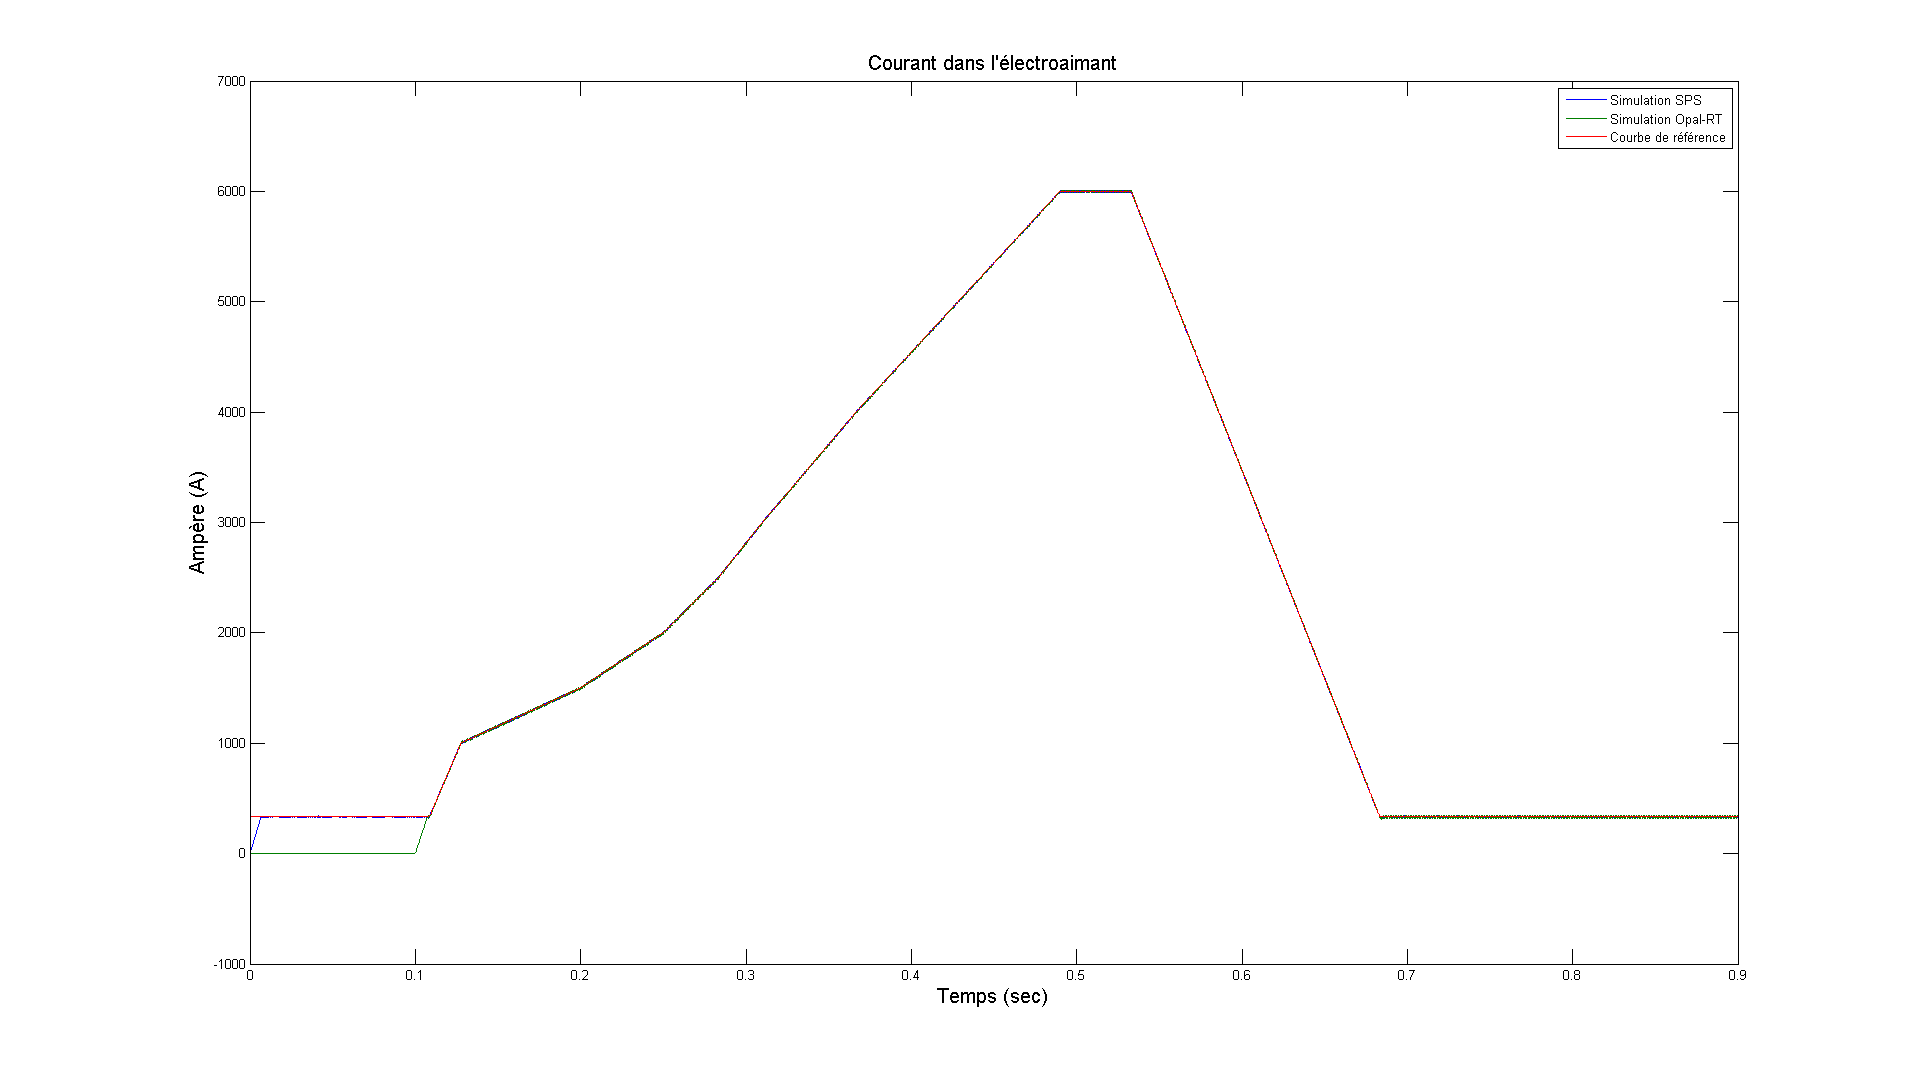
\includegraphics[width=0.95\textwidth]{fig/Opal-RT_Courant.png}}
 \caption{Courant traversant la charge sur Opal-RT et SPS pour un pas de calcul de 25$\mu$s pour le hacheur 4 quadrants (Affichage de 0.9 seconde)}
 \label{DC_ch_H4Q_1}
 \end{figure}

  \begin{figure}[htb]
 \centering
 \makebox[\textwidth][c]{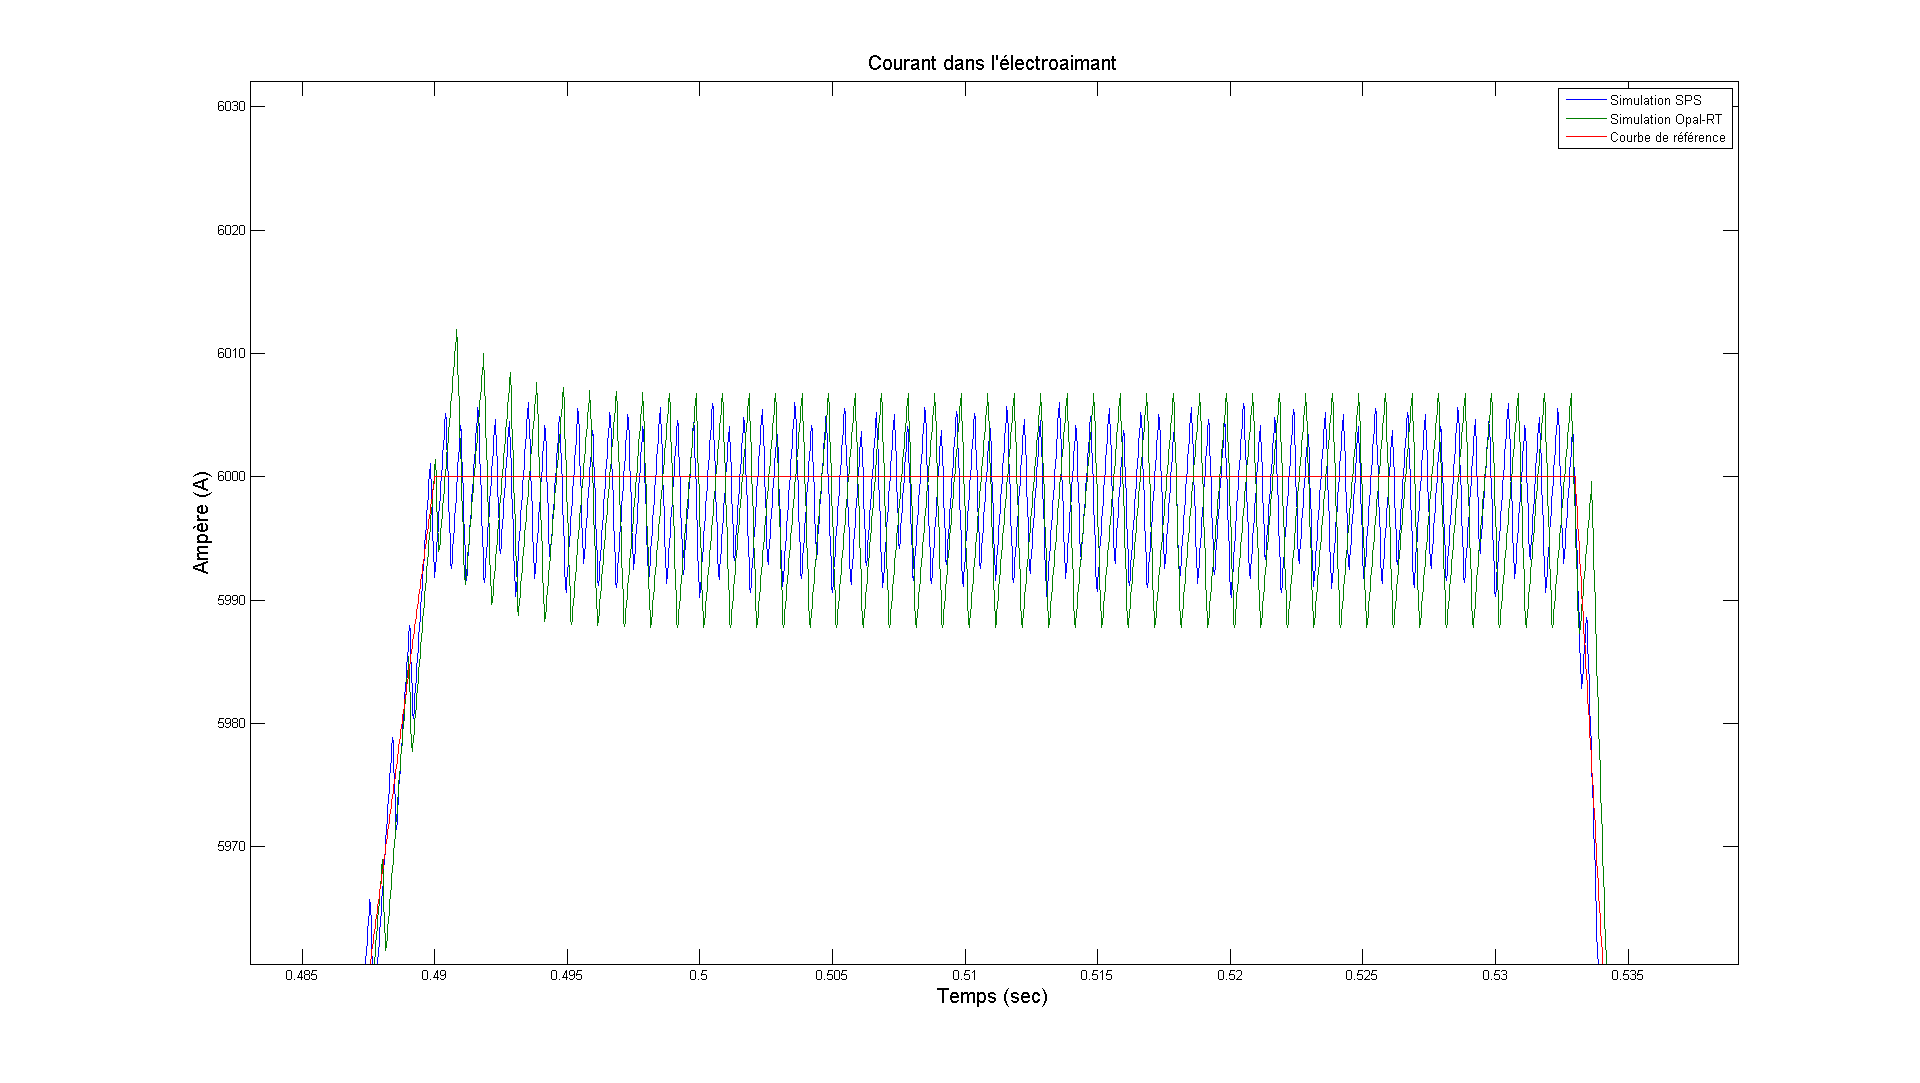
\includegraphics[width=0.95\textwidth]{fig/Opal-RT_Courant2.png}}
 \caption{Courant traversant la charge sur Opal-RT et SPS pour un pas de calcul de 25$\mu$s pour le hacheur 4 quadrants (Affichage de 0.005 seconde)}
 \label{DC_ch_H4Q_2}
 \end{figure}






\chapter{Matrice de vérification}

\begin{figure}[htb]
\centering
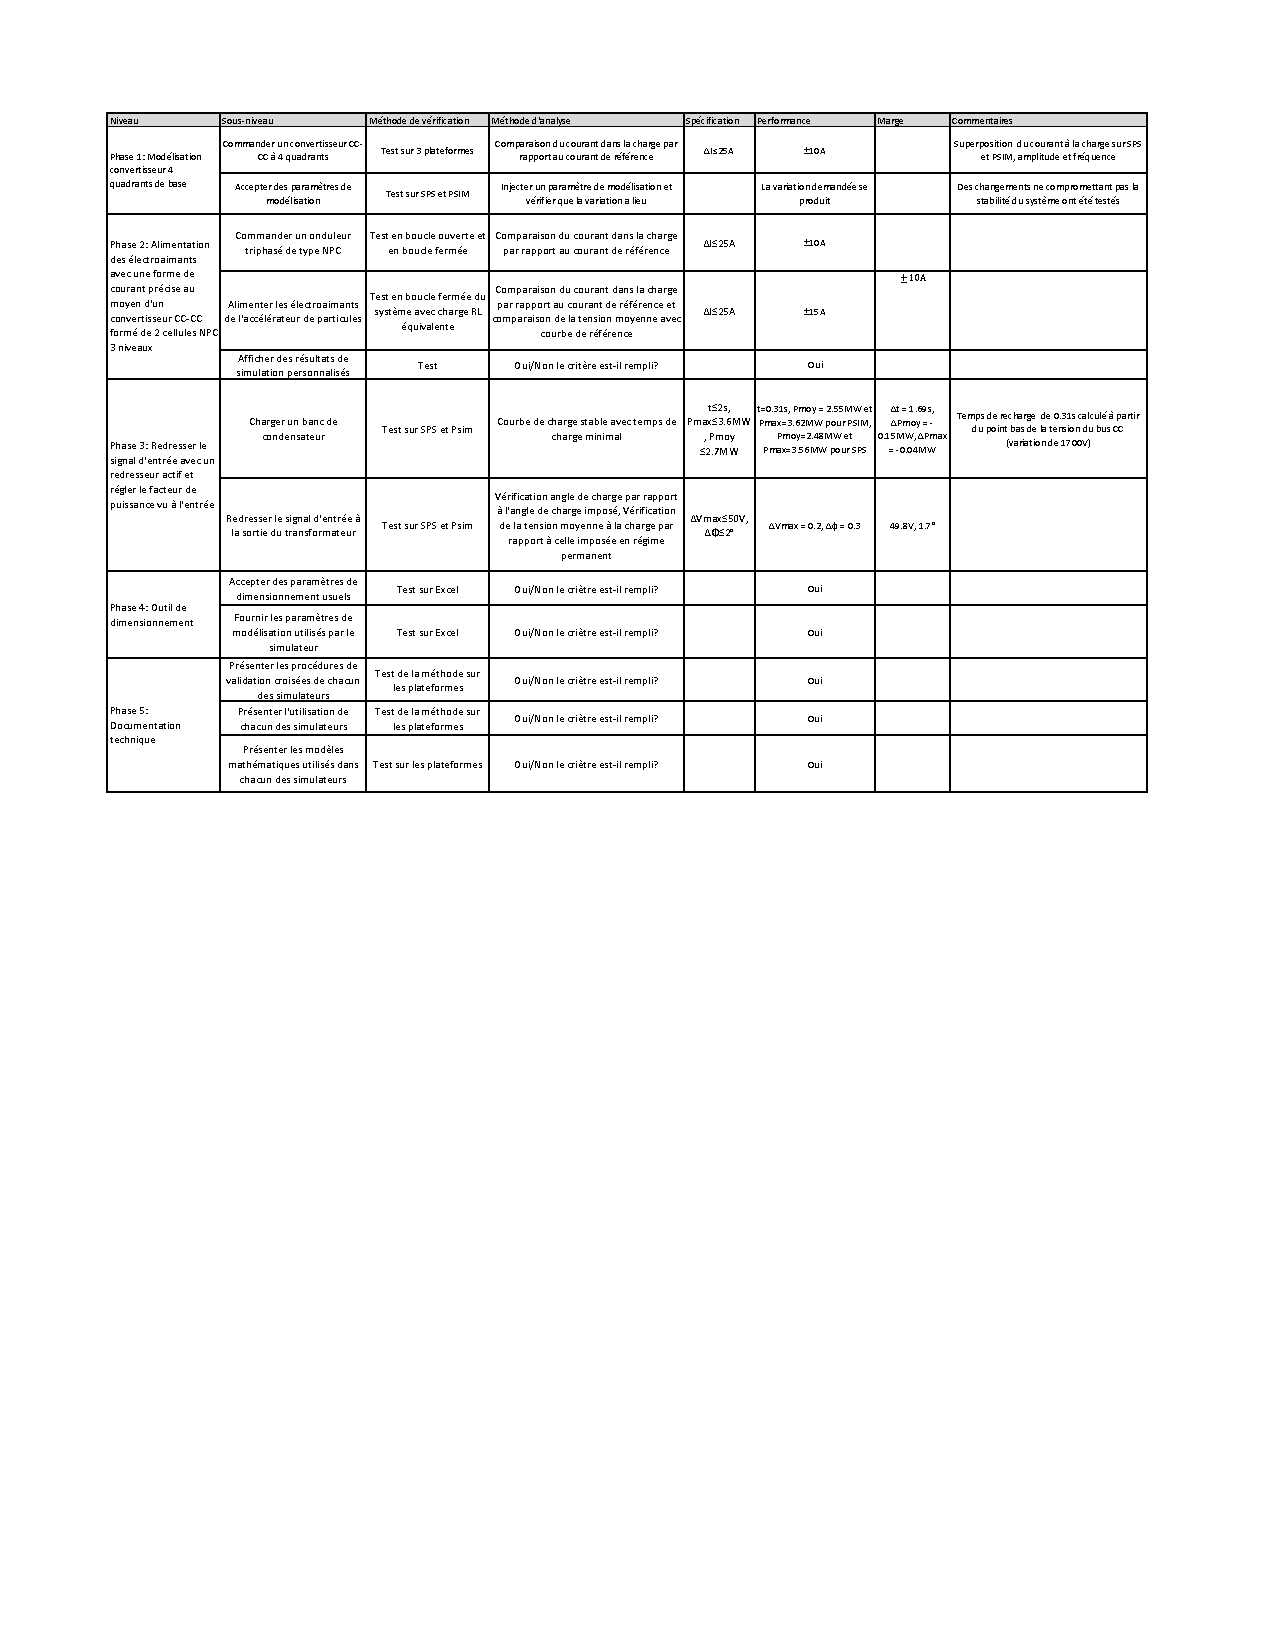
\includegraphics[scale=0.9,trim= 0mm 15cm 0mm 0mm, clip ]{matrice_verification.pdf}
\caption{Matrice de vérification}
\label{matrice}
\end{figure}
\chapter{Conclusion}
En somme, le projet portant sur la simulation d'un accélérateurs de particules fut un succès. Le cahier des charges du client au niveau de la dynamique des simulateurs a été respecté. L'outil de dimensionnement livré permet de faire varier les paramètres dans les simulations et de les lancer. Les simulations sont représentatives du comportement observé au CERN, si l'on se réfère aux courbes qui ont été fournies par le client. Ils permettent de compléter le cahier des charges. La section portant sur le simulateur temps réel n'est pas complète suivant des retards dans la livraison et l'installation des simulateurs. Cependant, il a été possible de documenter l'installation et l'utilisation, ce qui pour le client était le plus important. Pour ce qui est des avancées possible dans le projet, il est évident que l'intégration du convertisseur \og Trim \fg{} présenté à la figure \ref{conv_CERN} doit être réalisée. Ce convertisseur permet l'emploi d'inductances de couplage de plus grande impédance et donc une ondulation moins élevée du courant de sortie. De plus, les contrôles utilisés dans le projet sont des contrôles classiques fait de régulateurs PID. Les régulateurs employés au CERN sont des régulateurs RST qui sont réalisés exclusivement dans un modèle discret. Ils permettent une souplesse de réglage supérieure ainsi qu'une optimisation des paramètres des réglages.


\begin{figure}[htb]
\centering
\makebox[\textwidth][c]{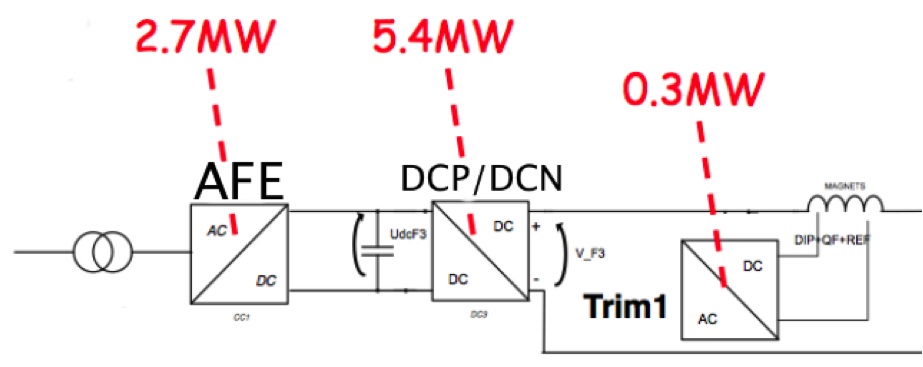
\includegraphics[scale=0.75]{fig/convertisseur_CERN.png}}
\caption{Schéma bloc de la chaîne de convertisseurs alimentant les électroaimants du CERN}
\label{conv_CERN}
\end{figure}


\end{document}
% Fin du document

